\documentclass[fleqn]{article}

\usepackage{mydefs}
\usepackage{notes}
\usepackage{url}
\usepackage{graphicx}

\begin{document}
\lecture{Computer Vision}{HW08: Decision trees, linear models}{Abhay Doke, UID: 29552668}

% IF YOU ARE USING THIS .TEX FILE AS A TEMPLATE, PLEASE REPLACE
% "CS 726, Fall 2011" WITH YOUR NAME AND UID.

Hand in via moodle at: \url{https://moodle.umass.edu/course/view.php?id=33024}.
Remember that only PDF submissions are accepted.  We encourage using
\LaTeX\ to produce your writeups.  See \verb+hw00.tex+ for an example
of how to do so.  You can make a \verb+.pdf+ out of the \verb+.tex+ by
running ``\verb+pdflatex hw00.tex+''.

% ANY LINE BEGINNING "%" IS A COMMENT.  YOU CAN UNCOMMENT THE BELOW
% TEXT AND FILL IN YOUR OWN.
% \begin{solution}
% \end{solution}
\bee
\i How many decision trees are there with three binary attributes and two class labels? With four binary attributes? 
\begin{solution}
For three binary attributes, dataset has at max $2^3$ instances and every instance can have one of the two labels. So there are $2^{2^{3}} = 256$ number of possible decision trees.
For four binary attributes, dataset has at max $2^4$ instances and every instance can have one of the two labels. So there are $2^{2^{4}} = 65536$ number of possible decision trees.  
\end{solution}

\vspace{1.5in}


\i Explain why the squared loss is not suitable for binary classification problems.	
\begin{solution}
For the binary classification problems the squared loss has slower convergence rate than the logistic loss or the hinge loss. For example a score vector is [0.4, 0, 0.6, 0] and the true class value distribution is [0, 0, 1, 0] with the third class being the correct class label.
The squared loss in this case is $(0.4 - 0)^{2} + (0 - 0)^{2} + (0.6 - 1)^{2} + (0 - 0)^{2} = 0.32$. Now during the updates, the training model will try to adjust the weight distribution with lower squared loss. This update can be [0.2, 0, 0.8, 0] which is  desired update or it can be [0.2, 0, 0.6, 0.2] which also gives the squared loss below 0.32. This makes convergence very slow because it does not know which is correct class score and considers only the sum of squared values of differences between score values and actual class distribution. Logistic loss or the hinge loss knows about the correct class score and they calculate the loss with respect to it and hence they have much faster convergence rates than the squared loss in the binary classification problems.    
\end{solution}
\vspace{1.5in}

\i A common way to get rid of having to deal with the threshold separately on a perceptron is to add a
new feature. This feature always has value one, and you learn a weight for it. Thus, if you have a 100
dimensional problem with a threshold, we solve it as a 101 dimensional problem with threshold at zero.
Draw a picture for one dimensional data and a linear separator with a (non-zero) threshold and draw
the corresponding picture for the same data, "lifted" into two dimensions, with the corresponding linear
separator with threshold zero. (Please make sure that the two separators are actually equivalent!)
\begin{solution}
\begin{center}
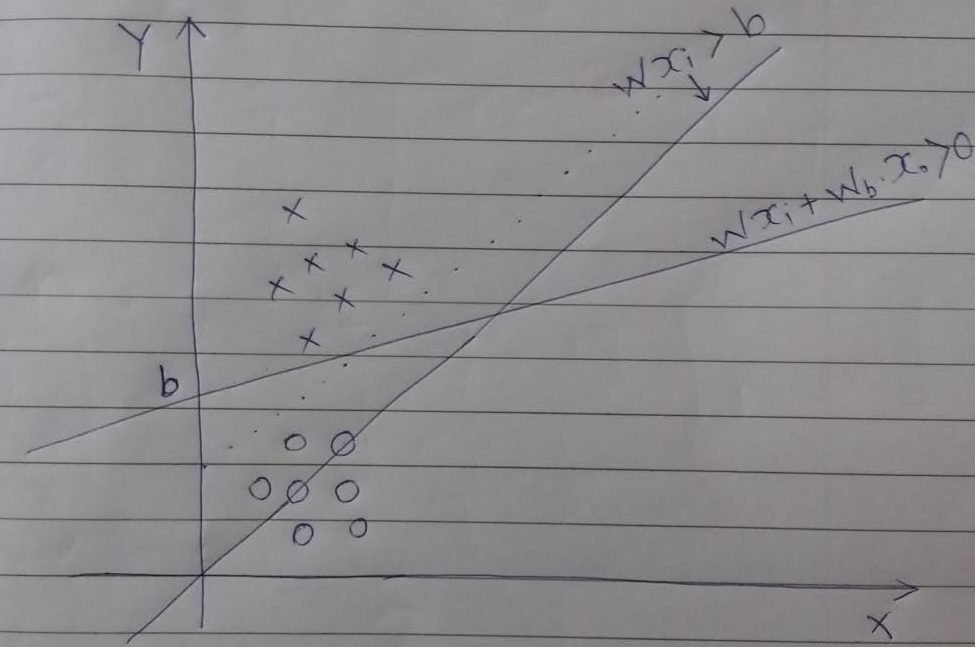
\includegraphics[width=0.9\textwidth]{graph.png}
\end{center}

The line which goes through the origin is the one with the non-zero threshold. So if b is the threshold then all the data points with class label 'x' have values $W.X > b$ and the data points with class label 'o' have $W.X < b$.
Now if we add this bias as a feature with it's value clamped to 1 and learn a weight for it, new model learns this value of 'b' and the separating line shifts to 'b' where the data points with class label 'x' have values 
$W_{new}.X_{new} > 0$ and the data points with class label 'o' have $W_{new}.X_{new} < 0$.
\end{solution}

\ene

\end{document}
